%\section{Motivación}
%\begin{frame}\frametitle{Motivación}
%
%    \begin{center}
%        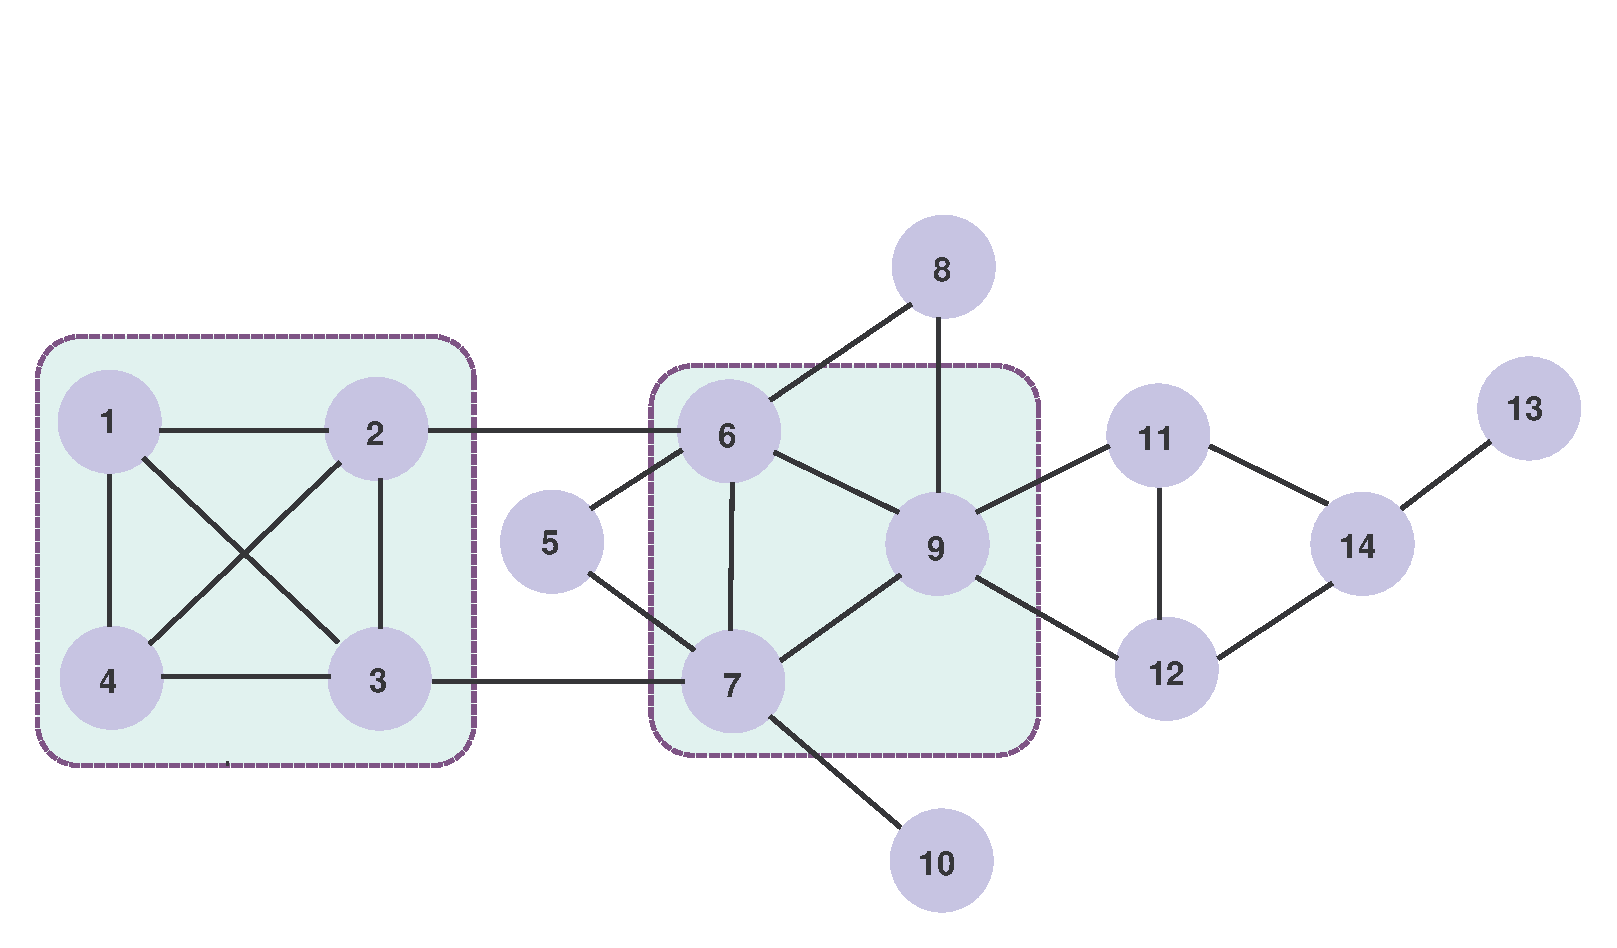
\includegraphics[scale=0.30]{figuras/martinsMCC}
%    \end{center}
%    \begin{tiny}    
%    \begin{block}{Observaciones}
%        \begin{itemize} 
%            \item Densidad de la estructura de vecindad de los cliques
%            \item Componente altamente relacionada con el resto del grafo.           
%            \item Gran cantidad de cliques máximo.            
%        \end{itemize}
%    \end{block}
%    \end{tiny}
%\end{frame}

\section{Problema}

%$\mathcal{G}$
%\emph{Clique} $\mathcal{C}$ 
%Currently, the backbone of the Internet infrastructure is supported by
%ber-optics communication. Fiber-To-The-Home (FTTH) services have a large
%penetration throughout the world, and provides high data rates to the nal
%customers. However, there are several shortcomings that should be addressed
%urgently. The physical design of FTTH is not suitable for large-scale natural
%disasters and/or malicious attacks [16]. The monitoring and detection of
%failures are sometimes slow, and a service disruption of hours is extremely
%harmful for business models. Furthermore, FTTH services are suering the
%capacity crunch problem, and elastic optical networks (EON) combined with
%smart trac engineering and additional redundancy is currently in order.
%Consequently, a smart augmentation of the physical network is mandatory.
%Since the deployment of ber-optics is an important economical investment,
%Reliability analysis deals with probabilistic failures on the components of a
%system. The reliability is precisely the probability of correct operation of the
%whole system, subject to random failures. Here, we consider a realistic hostile
%model, where both nodes and links could fail. Our goal is to understand the cost-
%reliability trade-off, and how the reliability is naturally increased adding levels
%of redundancy between distinguished terminals.
\subsection{Motivación}
\begin{frame}%\frametitle{Motivación}
%Generalized Steiner Problem with Node-Connectivity Constraints and
%Hostile Reliability (GSPNCHR)
    \begin{block}{Motivación}
    \begin{itemize} 
    	\item Los servicios de fibra al hogar (Fiber-To-The-Home - FTTH) tienen una gran penetración mundial brindando a los clientes finales transferencias de datos a altas velocidades.
    	\item La cantidad de aplicaciones y servicios sobre internet ha crecido exponencialmente.
    	\item Es mandatorio escalar de forma inteligente la infraestructura de red.
    	\item Dado que el despligue de la fibra optica es una importante inversión económica, el diseño topologico de las redes FTTH debe continuar considerandose.
	\end{itemize} 
    \end{block}
    %\begin{center}
    %    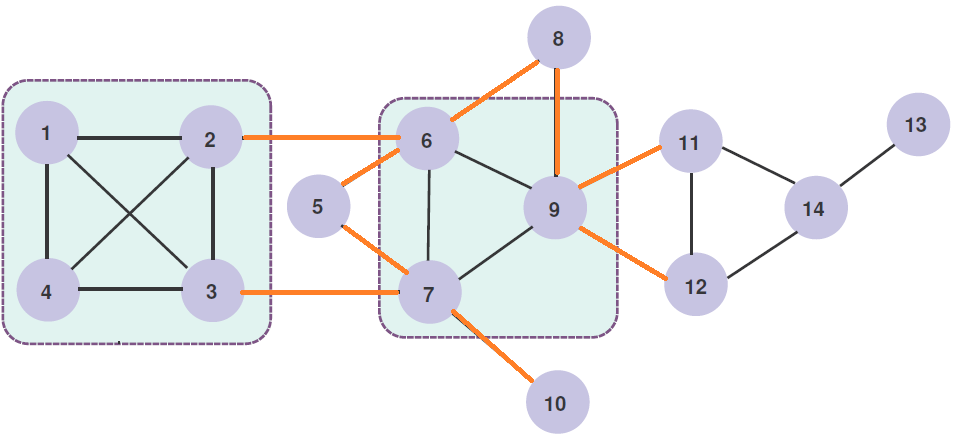
\includegraphics[scale=0.35]{figuras/martinsMod2}
    %\end{center}
\end{frame}

\subsection{Objetivos 1}
\begin{frame}%\frametitle{Objetivos 1}
    \begin{block}{Objetivos 1}
	\begin{itemize} 
    	\item Problema de optimización combinatoria motivado por el diseño topolóogico de redes de comunicaciones 
de sistemas, con restricciones de confiabilidad.
		\item El objetivo es interconectar nodos distinguidos, llamados terminales, utilizando un nivel adecuado de redundancia y de forma simultanea, satisfacer las restricciones de confiabilidad.
	\item En el análisis de confiabilidad nos enfrentamos a fallas aleatorias en los componentes del sistema. Es precisamente la probabilidad del correcto funcionamiento del sistema completo, sujeto a fallas aleatorias. Aquí se considera el modelo realista hostil, donde tanto nodos como aristas pueden fallar.
	\end{itemize} 
    \end{block}
\end{frame}

\subsection{Objetivos 2}
\begin{frame}%\frametitle{Objetivos 2}
    \begin{block}{Objetivos 2}
	\begin{itemize} 
    	\item Find a minimum-cost solution, meeting a reliability threshold, where both nodes and links may fail with given probabilities.
		\item Entender el trade-off entre costo-confiabilidad, y como la confiabilidad aumenta naturalmente agregando niveles de redundancia entre los nodos terminales.
    	\item Pertenece a la clase de problemas NP-Hard.
    	\item Como consecuencia, desarrolle una solución que resuelve de forma apróximada con una metodología GRASP/VNS la parte de optimización y para el análisis de la confiabilidad el método RVR.
	\end{itemize} 
    \end{block}
\end{frame}

%Our goal is to find a minimum-cost solution,
%meeting a reliability threshold, where both nodes and links may fail
%with given probabilities.
\subsection{Definición}
\begin{frame}\frametitle{Generalized Steiner Problem with Node-Connectivity Constraints and
Hostile Reliability (GSPNCHR)}
%    \begin{block}{}
    \begin{definition}[GSPNCHR]
Consider a simple undirected graph $G=(V,E)$, terminal-set $T \subseteq V$, link-costs $\{c_{i,j}\}_{(i,j) \in E}$ 
and connectivity requirements $R=\{r_{i,j}\}_{i,j \in T}$. Further, we assume that both links and non-terminal (Steiner) nodes 
fail with respective probabilities $P_E=\{p_e\}_{e\in E}$ and $P_{V-T}=\{p_v\}_{v\in V-T}$. 
Given a reliability threshold $p_{min}$, the goal is to build 
a minimum-cost topology $G_S \subseteq G$ meeting both the connectivity requirements 
$R$ and the reliability threshold: $R_{K}(G_S) \geq p_{min}$, being $K=T$ the terminal-set.
\end{definition}
 %   \end{block}
\end{frame}

\section{Estado del arte}
\subsection{Publicaciones Externas}
\begin{frame}\frametitle{Publicaciones}
\begin{block}{Publicaciones}
	\begin{enumerate}
	
	 \begin{small}
	\item Martins, P.(2012). \textbf{Cliques with maximum/minimum edge neighborhood and neighborhood density}. Computers And Operations Research, 39(3):594-608.	
	\item Martins, P., Ladrón, A. and Ramalhinho, H. (2014). \textbf{Maximun cut-clique problem: ILS heuristics and a data analysis application}. International Transactions in Operational Research, 22(5):775-809.	
	\item Gouveia, L. and Martins, P.(2015). \textbf{Solving the maximum edge-weigth clique problem in sparse graphs with compact formulation}. Journal on Computational Optimization, 3(1):1-30.		
	\end{small}
	\end{enumerate}
\end{block}
\end{frame}

\subsection{Publicaciones Locales}
\begin{frame}\frametitle{Publicaciones}
\begin{block}{Publicaciones Locales}
	\begin{enumerate} \begin{small}
	\item Bourel, M., Canale, E., Robledo, F., Romero, P., and Stábile, L. (2018a). \textbf{Complexity and Heuristics for the Max Cut-Clique Problem}. In International Conference on Variable Neighborhood 			Search. ICVNS 2018. Lecture Notes in Computer Science, vol. 11328. Springer, pages 28-40.
	\item Bourel, M., Canale, E., Robledo, F., Romero, P., and Stábile, L. (2018b). \textbf{A GRASP/VND 				Heuristic for the Max Cut-Clique problem}. In International Conference on Machine Learning, 					Optimization, and Data Science. Lecture Notes in Computer Science, vol. 11331. Springer, pages 357-367.
	\item Bourel, M., Canale, E., Robledo, F., Romero, P., and Stábile, L. (2019). \textbf{Complexity and Heuristics for the Weighted Max Cut-Clique Problem}. International Transactions in Operational Research. Under revision to be published.
	\end{small}
	\end{enumerate}
\end{block}
\end{frame}


\section{Complejidad}
\begin{frame}\frametitle{Complejidad}
\begin{proposition}
El problema MCC pertenece al conjunto de problemas $\mathcal{NP}$-Completos.
\end{proposition} 
\begin{proof}
Reducción desde $MAX$ -$CLIQUE$. 
\end{proof}

  \begin{center}
        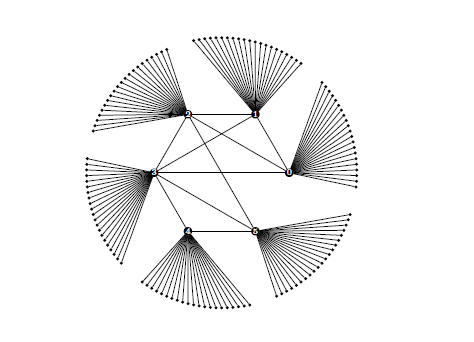
\includegraphics[scale=0.50]{figuras/Solucion/grafoHM}
 \end{center}
\end{frame}

\section{Solución}
\subsection{Algoritmo Genético}
\begin{frame}\frametitle{Algoritmo Genético}
\begin{small}
Por la complejidad inherente al problema, se presenta una solución basada en Algoritmos Genéticos.
\end{small}

    \begin{block}{Algoritmos Genéticos}
    \begin{small}
    
    $1$ - $Initialize(P_0)$;\\ 
    $2$ - $generation = 0$;\\	
    $3$ - $While$ $(not stopCriteria)$;\\		
	$4$ - 	$\hspace{6mm} evaluate (P(generation))$;\\
	$5$ - 	$\hspace{6mm} parents \gets selection (P(generation))$;\\
	$6$ - 	$\hspace{6mm} offspring \gets evolutiveOperators (parents)$;\\
	$7$ - 	$\hspace{6mm} newpop \gets replacement (offspring,P(generation))$;\\
	$8$ - 	$\hspace{6mm} generation ++ $;\\
	$9$ - 	$\hspace{6mm} P(generation) \gets newpop$;\\
	 		$Return$ $Best Solution Ever Found$;\\
	\end{small}
	
	%\begin{algorithm}[!h]
	%\caption{\textsc{GA Algorithm}} \label{alg:GABasic}	
%	\begin{algorithmic}[1]
%		\State {$Initialize(P_0)$;}
%		\State {$generation = 0$;}	
%		\While {$(not stopCriteria)$}
%		\State {$evaluate (P(generation))$;}
%		\State {$parents \gets selection (P(generation))$;}
%		\State {$offspring \gets evolutiveOperators (parents)$;}
%		\State {$newpop \gets replacement (offspring,P(generation))$;}
%		\State {$generation ++ $;}
%		\State {$P(generation) \gets newpop$;}
%		\EndWhile 		
%		\Return	{$Best Solution Ever Found$;}	
%	\end{algorithmic}
	%\end{algorithm}
    \end{block}
\end{frame}

%\subsection{Inicializacion de Soluciones y Criterio de Parada}
%\begin{frame}\frametitle{Inicialización y Criterio de Parada}
%	\begin{itemize}
%		\item Inicialización de soluciones, mediante proceso aleatorio de forma de otorgar diversidad.
%		\item Criterio de Parada, que la población evolucione durante 1000 generaciones.
%	\end{itemize}	    
%\end{frame}

\subsection{Diseño}
\begin{frame}\frametitle{Diseño de la solución}
\begin{center}
        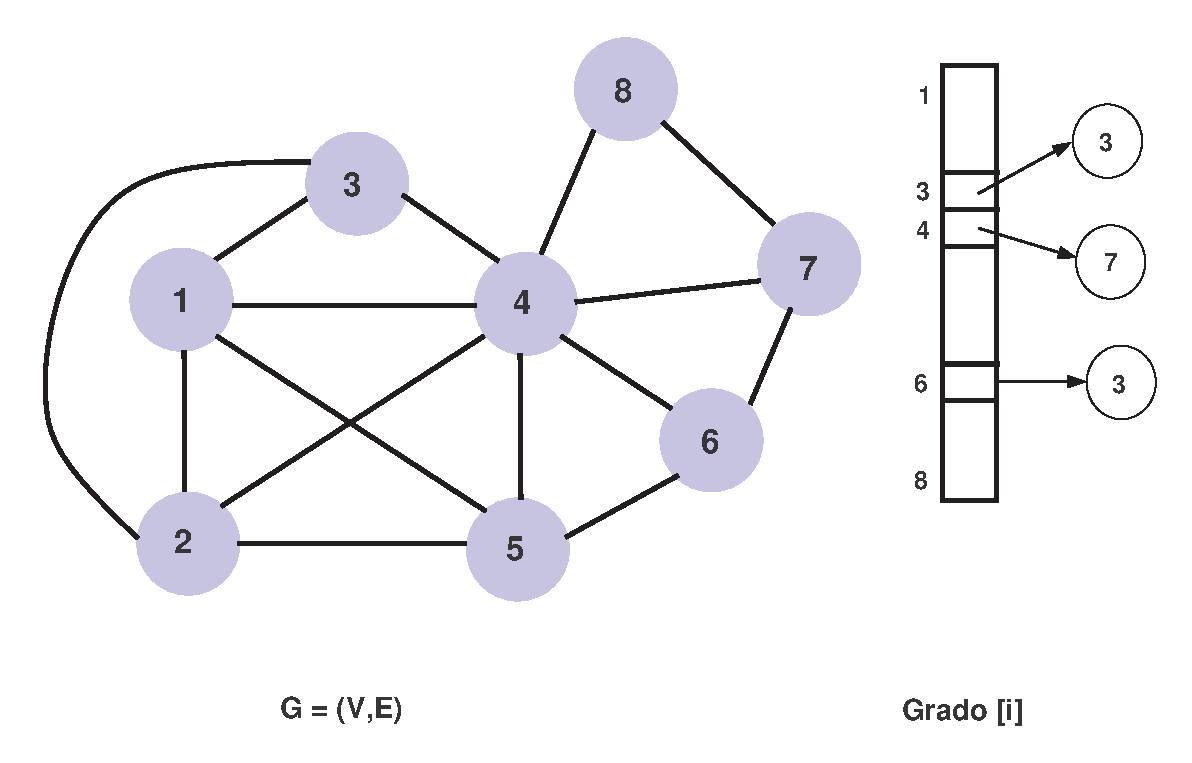
\includegraphics[scale=0.35]{figuras/Solucion/chap5_fig1}
\end{center}
\begin{itemize}
 \item Implementado en C++, biblioteca MALVA.
 \item Énfasis en la performance del algoritmo.
\end{itemize} 
\end{frame}

\subsection{Representación}
\begin{frame}\frametitle{Representación de la solución}

    %\begin{block}{Representación}
    \begin{small}
    Las soluciones factibles del problema, son todos los cliques que se encuentren en $\mathcal{G}= (V,E)$. \\
    Para representar un clique se define una tupla binaria de largo $n = |V|$, como: 
   
	\begin{displaymath}
    	X_{i} = 
    	\begin{cases}
      		1 & \text{si nodo } i \in \mathcal{C}\\
      		0 & \text{en otro caso}
    	\end{cases} \text{, } \forall i \in V 
	\end{displaymath}
    %\end{block}
    \end{small}
   	\begin{center}
    		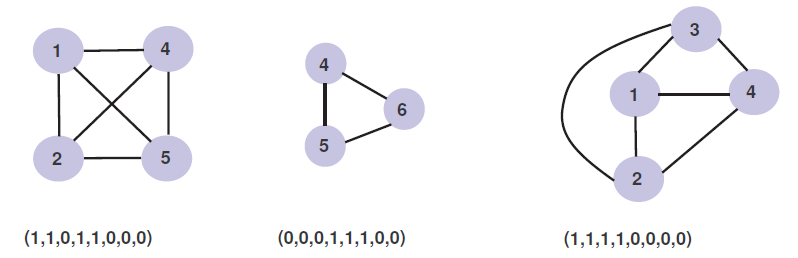
\includegraphics[scale=0.5]{figuras/Solucion/representacionSol}
    \end{center}
\end{frame}

\subsection{Función de Fitness}
\begin{frame}\frametitle{Función de Adecuación}
\begin{itemize}
\item Coincide con la función objetivo  
\item Busca maximizar la cantidad de aristas en el corte generado por el clique $\mathcal{C}$
\end{itemize}
%Coincide con la función objetivo y busca maximizar la cantidad de aristas en el corte generado por el clique $\mathcal{C}$\\

    \begin{block}{Función de Fitness} 
	%\begin{equation}	
	$	
	|\delta(\mathcal{C})| = \sum_{v \epsilon \mathcal{C}} deg(v) - |\mathcal{C}|\times|\mathcal{C}-1|$  
	%\end{equation}	\Delta
    \end{block}
\end{frame}

\subsection{Operadores Evolutivos}
\begin{frame}\frametitle{Cruzamiento}
  
	 Cruzamiento de 2 puntos
		
	\begin{center}
    	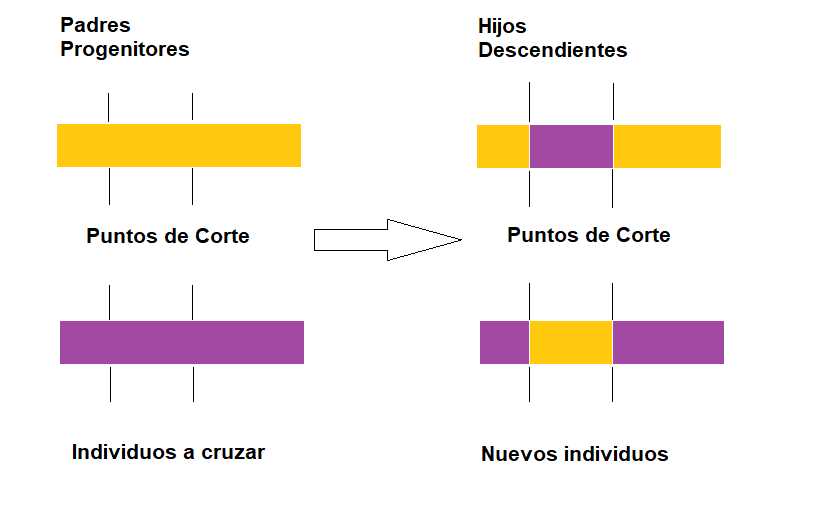
\includegraphics[scale=0.35]{figuras/Solucion/cruza2xP3}
    \end{center}     
\end{frame}

%\subsection{Operadores Evolutivos}
\begin{frame}\frametitle{Mutación}
 
	Mutación Simple
		
	\begin{center}
    	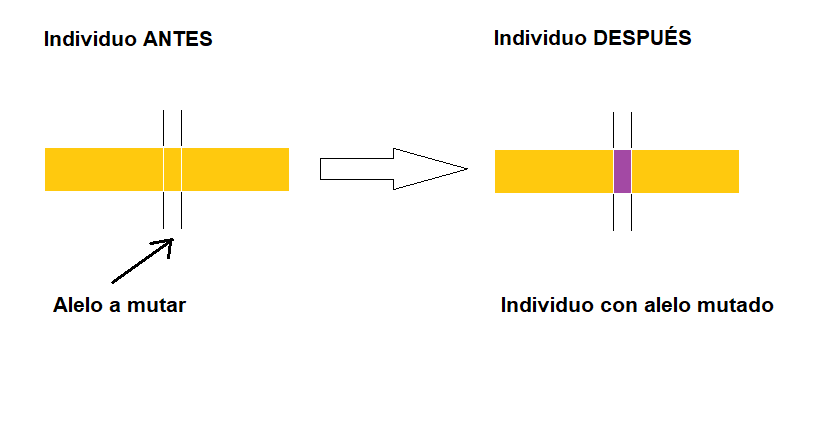
\includegraphics[scale=0.35]{figuras/Solucion/mutaSimple}
    \end{center}       
\end{frame}

%\begin{frame}\frametitle{Selección}
% 
%	Selección por Torneo de tamaño 2		
%	       
%\end{frame}



\subsection{Soluciones no factibles}
\begin{frame}\frametitle{Tratamiento}
  %Dada la naturaleza del problema y la representación elegida; las soluciones tienen alta probabilidad de ser NO FACTIBLES. 
  %Algoritmo de corrección inspirado en la etapa de Construcción de las Metaheuristicas utilizadas.
  %Tratamiento de soluciones no factibles.  
  Se utiliza algoritmo de corrección basado en la etapa de construcción del GRASP/VND, luego de las siguiente etapas.\\
%    \begin{center}
%    	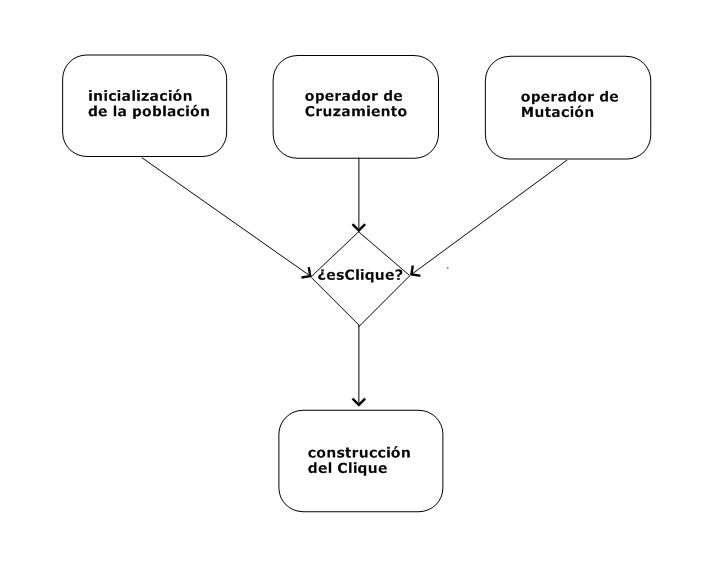
\includegraphics[scale=0.50]{figuras/Solucion/diagrama55}
%    \end{center} 
%\textbf{¿Cuándo?}\\
  \begin{itemize}
  \item inicialización la población
  \item aplicación del operador de Cruzamiento
  \item aplicación del operador de Mutación
  \end{itemize}  
\end{frame}

\subsection{Calibración}
\begin{frame}\frametitle{Ajuste de Parámetros}
\begin{itemize}
\item Algoritmos genéticos son NO deterministas
\item Test estadísticos para reportar: calidad y eficiencia computacional.
\end{itemize}

\begin{small}
\textbf{Instancias utilizadas}
\end{small}
\begin{table}[h!]
\centering
%\caption{Instancias para ajuste de parámetros.}
%\label{tab:ajusteParam}
\scalebox{0.7}{
\begin{tabular}{|l|c|c|c|c|}
  \hline
  \textbf{Instancia} & \textbf{$|V|$} & \textbf{$|E|$} & \textbf{Densidad} & $|E(C)|$\\
  \hline
  p\_hat300-1 & 300 & 10933 & 0.244 & 789\\
  MANN\_a9 & 45 & 918 & 0.9273 & 412\\
  keller4 & 171 & 9435 &0.649 &1140\\ 
  \hline
\end{tabular}}
\end{table}

%\begin{small}
%\begin{itemize}
%\item obtener valores óptimos para todas las configuraciones 
%\emph{$pop \times p_{cross} \times p_{mutex} \times$ instancia} $(3\times 3\times 3\times 3)\times 30= 2430!!!!$
%\item para cada configuración rankear el resultado, compararlo con resultado de otras configuraciones
%\item elegir la configuración que mejor rankee, por dimensión o comparando todas contra todas.
%\end{itemize}
%\end{small}

\begin{small}
\textbf{Resultado de la calibración}
\end{small}

\begin{table}[h!]
\centering
\label{tab:resultAjuste}
\scalebox{0.7}{
\begin{tabular}{|l|c|}
  \hline
  \textbf{Parámetro} & \textbf{Valor}\\
  \hline
  tamaño población  & 200 \\
  prob. cruzamiento & 0.8 \\
  prob. mutación	& 0.1 \\ 
  \hline
\end{tabular}}
%\caption{Resultado de la calibración.}
\end{table}
\end{frame}

\section{Resultados}
\subsection{Resultados I}
\begin{frame}\frametitle{Instancias de prueba}
\textbf{Caracterización instancias}
\begin{table}[h!]
	\hspace{-1cm}
	%\centering
	\scalebox{0.7}{  
	\begin{tabular}{l|rrrr}
		\hline
		{Instancias} & \multicolumn{4}{c}{Características de las instancias} \\
		%\cline{1-3} \cline{5-11} 
		 & $|V|$ & $|E|$ & Densidad & $|E(C)|$\\
		\hline
		c-fat200-1 	&200 	&1534	&0.071 	&81\\
		c-fat200-2 	&200 	&3235 	&0.163 	&306\\
		c-fat200-5 	&200 	&8473 	&0.426 	&1892\\
		c-fat500-1 	&500 	&4459 	&0.036 	&110\\
		c-fat500-2 	&500 	&9139 	&0.073 	&380\\
		c-fat500-5 	&500 	&23191 	&0.186 	&2304\\
		c-fat500-10 &500 	&46627 	&0.374 	&8930\\
		%p\_hat300-1	&300 	&10933	&0.244 	&789\\		
		p\_hat300-2 &300 	&21928 	&0.489 	&4637\\
		p\_hat300-3 &300 	&33390 	&0.744 	&7740\\
		%keller4 	&171 	&9435 	&0.649 	&1140\\
		keller5 	&776 	&225990 &0.752 	&15184\\
		%MANN\_a9 	&45 	&918 	&0.9273	&412\\
		MANN\_a27 	&378 	&70551 	&0.990 	&31284\\
		c125\_9 	&125 	&69632 	&0.899 	&236406\\	
		\hline
	\end{tabular}}	
\end{table}
\end{frame}

%\subsection{Resultados II}
%\begin{frame}\frametitle{Resultados obtenidos}
%
%\begin{table}[h!]
%	\hspace{-1cm}
%	\scalebox{0.7}{
%	\begin{tabular}{lrr|r|rrr|r}
%		\hline
%		\multicolumn{3}{c}{\textbf{Características}}& \textbf{ILS}  & \multicolumn{3}{l}{\textbf{Algoritmo Genético}}& \textbf{GAP} \\
%		%\cline{1-3} \cline{5-11} 
%		Instancias & $|V|$ & Densidad & $|E(C)|$ & Mejor & Prom. & T(s) prom. &(\%)\\
%		\hline
%		c-fat200-1 	&200  	&0.071 	&\textbf{81} 	&\textbf{81} 	&81 		&6.4	&0.0\\
%		c-fat200-2 	&200	&0.163	&\textbf{306} 	&\textbf{306} 	&306 		&7.5	&0.0\\
%		c-fat200-5 	&200	&0.426	&\textbf{1892} 	&\textbf{1892} 	&1892 		&12.5	&0.0\\
%		c-fat500-1 	&500	&0.036	&\textbf{110} 	&\textbf{110} 	&110 		&16.15	&0.0\\
%		c-fat500-2 	&500	&0.073	&\textbf{380} 	&\textbf{380} 	&380 		&14.3	&0.0\\
%		c-fat500-5 	&500	&0.186	&\textbf{2304} 	&\textbf{2304} 	&2304 		&20.36	&0.0\\
%		c-fat500-10 &500	&0.374	&\textbf{8930} 	&\textbf{8930} 	&8930 		&32.59	&0.0\\
%		p\_hat300-2 &300	&0.489	&\textbf{4637} 	&\textbf{4637} 	&4633.40 	&171.9	&0.0\\
%		p\_hat300-3 &300	&0.744	&\textbf{7740} 	&\textbf{7740} 	&7387.27 	&279.8	&0.0\\
%		c125\_9 	&125	&0.899	&\textbf{2766} 	&\textbf{2766} 	&2737.2 	&5.0	&0.0\\
%		keller5 	&776	&0.752	&\textbf{15184} &\textbf{13120} &12382 		&50.57	&0.16\\
%		MANN\_a27 	&378	&0.990	&\textbf{31284} &\textbf{30570} &30405 		&46.49	&0.02\\		
%		\hline
%	\end{tabular}}	
%	%\caption{Resultados obtenidos para el Máximo Clique-Corte.} \label{table:resultados}
%\end{table}
%\end{frame}

\subsection{Resultados II}
\begin{frame}\frametitle{Resultados obtenidos}
\begin{table}[h!]
	%\hspace{-1cm}
	\scalebox{0.7}{ 
	\begin{tabular}{l|rr|rr|r}
		\hline
		\multicolumn{1}{l}{} & \multicolumn{2}{c}{\textbf{GRASP/VND}} & \multicolumn{2}{l}{\textbf{Algoritmo Genético}} & GAP \\
		%\cline{1-3} \cline{5-11} 
		Instancias & $|E(C)|$ prom. & $T(s)$ prom. & $|E(C)|$ prom. & $T(s)$ prom. &(\%) \\
		\hline
		c-fat200-1 	&81 		&0.37 		&81 		&6.4	&0.0\\
		c-fat200-2 	&306 		&0.81 		&306 		&7.5	&0.0\\
		c-fat200-5 	&1892 		&4.94 		&1892 		&12.5	&0.0\\
		c-fat500-1 	&110 		&2.46 		&110 		&16.15	&0.0\\
		c-fat500-2 	&380 		&5.83 		&380 		&14.3	&0.0\\
		c-fat500-5 	&2304 		&10.85 		&2304 		&20.36	&0.0\\
		c-fat500-10 &8930 		&65.74 		&8930 		&32.59	&0.0\\
		p\_hat300-2 &4636.2 	&3659.39 	&4633.40 	&171.9	&$\approx$0.0\\
		p\_hat300-3 &7726.8 	&3992.42 	&7387.27 	&279.8	&0.04\\
		c125\_9 	&2766 		&253.25	 	&2737.2 	&5.0	&0.01\\
		keller5 	&15183.24 	&1167.64 	&12382 		&50.57	&0.18\\
		MANN\_a27 	&31244.10 	&548.54 	&30405 		&46.49	&0.03\\		
		\hline
	\end{tabular}}	
\end{table}
\end{frame}


\section{Conclusiones}
\begin{frame} \frametitle{Conclusiones}
\begin{block} {Conclusiones}
   	\begin{itemize} 
   	\begin{small}     	
	\item Aplicaciones diversas en diferentes áreas.
	\item Se demuestra la $\mathcal{NP}$-Completitud.
	\item Solución competitiva con las existentes y con tiempos de ejecución muy buenos.   	
	\end{small} 	
 	\end{itemize} 	
 \end{block}
% 	\emph{Resumen:\\
% 	Se cuenta con una solución competitiva con soluciones existentes y con tiempo de ejecución muy buenos.}   
\end{frame}

\subsection{Trabajo Futuro}
\begin{frame} \frametitle{Trabajo Futuro}
\begin{block} {Trabajo Futuro}
 	 \begin{itemize}
 	 	\item Aplicaciones reales en grandes superficies.
 	 	\item Explorar la versión con pesos en las aristas, (WMCC).
 	 \end{itemize}  
 \end{block} 	   
\end{frame}

\subsection{Gracias}
\begin{frame} \frametitle{Fin}
\begin{huge}
Gracias por su atención.
\end{huge}

\end{frame}

%\section{Conclusiones}
%\begin{frame} \frametitle{Contributions}
%    \begin{itemize}
%    
%    \item The hardness for the \emph{MCC} was established [2]. 
%    \item A GRASP/VND heuristic was developed [1]. 
%    \item A bounding acceleration scheme was proposed [3].  
%    \item Results are competitive with state-of-the-art solutions [3]. 
%    \item A weighted version was also proposed [3]. 
%    
%%        \item \emph{MCC} belongs to the $\mathcal{NP}$-Complete set.
%%        \item The search space is reduced using bounds.
%%%        \item An exact Integer Linear Programming (ILP) formulation is proposed.
%%        \item A heuristic addressing this problem was developed.
%%        \item Results confirm that it is competitive with the state-of-the-art solutions.
%%        \item A further study including weights to each edge was proposed. This problem is known as \emph{Maximum Edge-Weight Neighborhood Clique} (MEWNC).
%    \end{itemize}
%\end{frame}